\documentclass[handout]{beamer}
\usepackage{pgfpages}
\pgfpagesuselayout{2 on 1}[a4paper,border shrink=5mm]

\usepackage{amsmath,amssymb,amsthm,array}
\usepackage{bm}
\usepackage{multirow}
\usepackage{multicol}
\usepackage{algorithm}
\usepackage{hyperref}
\usepackage{algorithmic}
\usepackage[normalem]{ulem}
\usepackage{fontspec}
\usepackage{numprint}

\setmainfont{CMU Serif}
\setsansfont{CMU Sans Serif}
\newfontfamily{\greekfont}{CMU Serif}
\newfontfamily{\greekfontsf}{CMU Sans Serif}

\usetheme{Rochester}
\usecolortheme{beaver}
 
\setbeamertemplate{navigation symbols}{}
\title{Κρυπτογραφικά Πρωτόκολλα}
\author{Παναγιώτης Γροντάς}
\date{05/12/2017}
\defbeamertemplate*{footline}{shadow theme}
{%
  \leavevmode%
  \hbox{
		\begin{beamercolorbox}[wd=.4\paperwidth,ht=2.5ex,dp=1.125ex,leftskip=.3cm,rightskip=.3cm plus1fil]{title in head/foot}%
			\usebeamerfont{title in head/foot} Cryptographic Protocols  %
		\end{beamercolorbox}
		\begin{beamercolorbox}[wd=.5\paperwidth,ht=2.5ex,dp=1.125ex,leftskip=.3cm,rightskip=.3cm plus1fil]{title in head/foot}%
			\usebeamerfont{title in head/foot} \hfill \insertsection  %
		\end{beamercolorbox}
		\begin{beamercolorbox}[wd=.1\paperwidth,ht=2.5ex,dp=1.125ex,leftskip=.3cm plus1fil,rightskip=.3cm]{author in head/foot}%
			\usebeamerfont{author in head/foot}\insertframenumber\,/\,\inserttotalframenumber
		\end{beamercolorbox}%
  }%
  \vskip0pt%
}

\institute{ΕΜΠ - Κρυπτογραφία - (2017-2018)}
 \hypersetup{
  pdfauthor={Panagiotis Grontas},
  pdftitle={Protocols},
  colorlinks=true,
  urlcolor=blue,
  linkcolor=white
}

\setlength{\columnseprule}{0.4pt}
\begin{document}
\newcommand{\xor}{ \oplus }
\newcommand{\msg}{ \mathtt{M} }
\newcommand{\KEY}{ \mathtt{K} }
\newcommand{\CPH}{ \mathtt{C} }
\newcommand{\keygen}{\mathtt{KeyGen}}
\newcommand{\enc}{\mathtt{Encrypt}}
\newcommand{\dec}{\mathtt{Decrypt}}
\newcommand{\sign}{\mathtt{Sign}}
\newcommand{\verify}{\mathtt{Verify}}
\newcommand{\adv}{$\mathcal{A}$ }
\newcommand{\Hash}{\mathcal{H} }
\newcommand{\advb}{$\mathcal{B}$ }
\newcommand{\chal}{$\mathcal{C}$ }
\newcommand{\cs}{$\mathcal{CS}$}
\newcommand{\Zed}{\mathbb{Z}} 
\newcommand{\zns}{\mathbb{Z}^*_n}
\newcommand{\zs}[1]{\mathbb{Z}^*_{#1}}

\newcommand{\green}[1]{\textcolor{teal}{#1}}
\newcommand{\Green}[1]{\textcolor{Teal}{#1}}
\newcommand{\ForestGreen}[1]{\textcolor{ForestGreen}{#1}}
\newcommand{\blue}[1]{\textcolor{blue}{#1}}
\newcommand{\magenta}[1]{\textcolor{magenta}{#1}}
\newcommand{\cyan}[1]{\textcolor{cyan}{#1}}

\newcommand{\twopartdef}[4]
{ 
		\begin{cases}
			#1 , #2 \\
			#3 , #4
		\end{cases} 
}

\begin{frame}
	\titlepage
\end{frame}
	
\begin{frame}{Περιεχόμενα}
\begin{itemize}
\item Ασφαλής Υπολογισμός Πολλών Συμμετεχόντων \pause 
\item Πρωτόκολλα
\begin{itemize}
	\item Πολλοί συμμετέχοντες
	\item Πολλά μηνύματα
\end{itemize}
\item Διαμοιρασμός Απορρήτων (secret sharing) \pause 
\item Μη συνειδητή μεταφορά (oblivious transfer) \pause
\end{itemize}
\end{frame}

\section{Secure Multi Party Computation}
\begin{frame}{Το πρόβλημα}
	\begin{itemize}
		\item $m$ παίκτες θέλουν να υπολογίσουν από κοινού την τιμή της συνάρτησης $f(x_1, x_2, \cdots x_m)$
		\item Κάθε παίκτης $P_i$ συνεισφέρει την είσοδο $x_i$
		\item Γενίκευση: κάθε παίκτης διαθέτει τη δική του συνάρτηση $f_i$, αλλά χρειάζεται είσοδο από όλους
		\item Μπορεί να γίνει;
		\begin{itemize}
			\item Χωρίς να αποκαλυφθεί καμία πληροφορία εκτός από το αποτέλεσμα
			\item Υποθέσεις ασφάλειας
			\item Πολυπλοκότητα: Υπολογισμών / Επικοινωνίας
		\end{itemize}
		\item Δεν είναι αποδεκτή η χρήση TTP
	\end{itemize}
\end{frame}

\section{Secret Sharing - Threshold Cryptosystems}
\begin{frame}{Διαμοιρασμός απορρήτων - Εισαγωγή}
Βασικό συστατικό Secure Multi Party Computation

\alert{Το πρόβλημα}\\
Κλειδιά: κρίσιμα κρυπτογραφικά δεδομένα (όχι τα μόνα)\\
\medskip
\pause
Για παράδειγμα: ιδιωτικό κλειδί
\begin{itemize}
\item Δύναμη αποκρυπτογράφησης
\item Δύναμη υπογραφής
\end{itemize}
\medskip
\pause
\green{Λύση}\\
Δεν θέλουμε να είναι στην φυσική κατοχή μίας οντότητας (μόνο)
\end{frame}

\begin{frame}{Additive secret sharing}
Έστω $(\mathbb{G},+)$ μια ομάδα και $s \in \mathbb{G}$ το μυστικό το οποίο θέλουμε να μοιράσουμε σε $n$ παίκτες

\begin{itemize}

\pause
\item Διαλέγουμε τυχαία $s_1, \cdots s_{n-1} \in \mathbb{G}$

\pause
\item Θέτουμε $s_n = s - \sum_{i=1}^{n-1} s_i$

\pause
\item Μοιράζουμε τα $\{ s_i \}_{i=1}^n$ στους παίκτες

\pause
\item Ανακατασκευή $s = \sum_{i=1}^n s_i$
\end{itemize}

\pause
\green{Παραλλαγή}: Αν $s \in \{0,1\}^l$ τότε υλοποίηση με XOR

\pause
\alert{Πρόβλημα:} Ένας παίκτης μπορεί να ακυρώσει την ανακατασκευή 
\end{frame}

\begin{frame}{Threshold Secret Sharing}
\blue{$(t,n)$ threshold secret sharing}
\begin{itemize}
\item Ένα μυστικό $s$ πρέπει να μοιραστεί σε $n$ παίκτες $P_1, P_2, \cdots P_n$ ώστε:
\pause
\begin{itemize}
\item Οποιοδήποτε υποσύνολο από τουλάχιστον $t+1$ παίκτες να μπορεί να το ανακτήσει
\pause
\item Κανένα υποσύνολο με $t$ παίκτες να μην μπορεί
\pause
\end{itemize}
\item \green{Υπόθεση} Εμπιστεύομαστε τον διανομέα $D$ και τους παίκτες
\end{itemize}
\end{frame}

\begin{frame}[allowframebreaks]{Shamir Secret Sharing}

\begin{block}{Πολυωνυμική παρεμβολή}
\begin{itemize}
\item Έστω ένα πολυώνυμο βαθμού $t$: $f(x) = a_0+a_1x+\cdots+a_tx^t$
\item Μπορεί να ανακατασκευαστεί από $t+1$ σημεία $(x_i,f(x_i))$ με διαφορετικές τετμημένες (με μοναδικό τρόπο)
\item Υπάρχουν άπειρα πολυώνυμα βαθμού $t$ που περνούν από $t$ τέτοια σημεία
\item Ανάκτηση πολυωνύμου: συντελεστές Lagrange
\item $\lambda_i(x) = \prod_{k=0, k \neq i}^t \frac{x-x_k}{x_i-x_k}$
\item Προκύπτει το $L(x) = \sum_{i=0}^t y_i \lambda_i(x) = y_0 \lambda_0(x) + y_1 \lambda_1(x) + \cdots y_t \lambda_t (x) $
\item Αποδεικνύεται ότι είναι μοναδικό δηλ: $L = f$
\end{itemize}
\end{block}
\framebreak

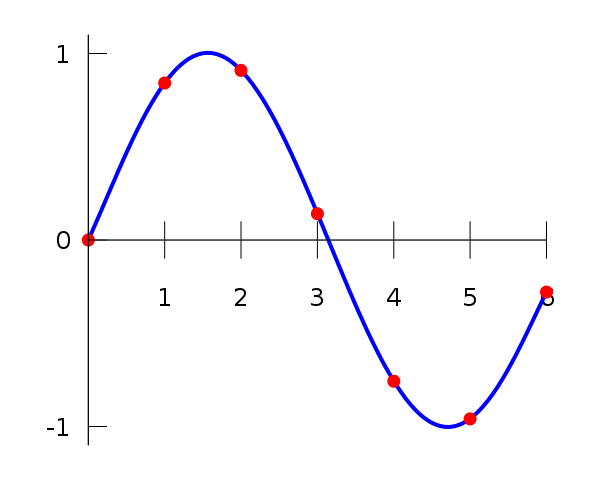
\includegraphics[scale=0.4]{polynomialinterpolation.png}

\framebreak

\begin{block}{Εφαρμογή στο διαμοιρασμό απορρήτων}
Υποθέτουμε ότι διαθέτουμε έναν έμπιστο διανομέα:
\begin{itemize}
\item Επιλέγει και δημοσιοποιεί ένα πρώτο $p$
\item Επιλέγει $t$ συντελεστές ενός πολυωνύμου βαθμού $t$ $\{a_t, \cdots, a_1 \} \in_R \mathbb{Z}_p$
\item Θέτει ως σταθερό όρο το μυστικό $s$
\item Προκύπτει το πολυώνυμο $f(x) = a_t \cdot x^t +  a_{t-1} \cdot x^{t-1} + \cdots + a_{1} \cdot x + s \pmod{p}$
\item $f(0)=s$
\item Μοιράζει στον παίκτη $i$ την τιμή $(i,f(i))$
\end{itemize}
\end{block}

\framebreak
\begin{block}{Ανακατασκευή}
\begin{itemize}
\item Παρατήρηση: Δεν μας ενδιαφέρει να υπολογίσουμε το πολυώνυμο $f$ αλλά το $f(0)$
\item Κάθε παίκτης $i$ υπολογίζει τους συντελεστές Lagrange
\item $\lambda_i(0) = \prod_{k=1, k \neq i}^{t+1} \frac{-k}{i-k} \bmod{p}$
\item $t+1$ παίκτες μπορούν να υπολογίσουν το $f(0)$ ως: $\sum_{i=1}^{t+1} f(i) \lambda_i(0) \bmod{p}$
\item Ανακτούν το μυστικό υπολογίζοντας το $p(0)$
\end{itemize}
\end{block}
\end{frame}

\begin{frame}{Παρατηρήσεις I}
\begin{itemize}
\item Πληροφοριοθεωρητική ασφάλεια αν ο αντίπαλος διαθέτει λιγότερα μερίδια
\pause
\item Μπορούν να προστεθούν εύκολα καινούρια μερίδια, χωρίς να αλλάξουν τα παλιά: Υπολογισμός νέων σημείων
\pause
\item Εύκολη αντικατάσταση μεριδίων: Υπολογισμός νέων σημείων (πρέπει να γίνει ασφαλής καταστροφή των παλιών)
\pause
\item Σημαντικοί παίκτες: περισσότερα από ένα μερίδια
\pause
\item Αλλαγή Μεριδίων: Τροποποίηση πολυωνύμου χωρίς να αλλάξει το μυστικό
\pause
\item Ομομορφικές ιδιότητες (άθροισμα πολυωνύμων είναι πολυώνυμο) \\
$s_1 + s_2 = f(0) + g(0) = (f+g)(0)$
\end{itemize}
\end{frame}

\begin{frame}{Παρατηρήσεις II}
\begin{itemize}
\item Μειονεκτήματα: Εμπιστοσύνη
\begin{itemize}
\item Κακόβουλος διανομέας: Λανθασμένα μερίδια σε τμήμα των παικτών 
\pause
\item Κακόβουλος παίκτης: Παροχή λανθασμένων μεριδίων κατά τη διάρκεια της ανακατασκευής
\pause
\end{itemize}
\item Λύση: Συνδυασμός με σχήμα δέσμευσης (Verifiable Secret Sharing)
\pause
\begin{itemize}
\item Ο διανομέας μαζί με τα μερίδια παρέχει και δεσμεύσεις για τους συντελεστές
\item Οι παίκτες επαληθεύουν ότι οι δεσμεύσεις δίνουν το σημείο τους
\end{itemize}
\end{itemize}
\end{frame}

\begin{frame}{Feldman Verifiable Secret Sharing}
\begin{block}{Υποθέσεις}
	\begin{itemize}
		\item Ομάδα $\mathbb{G}$ τάξης $q$ με γεννήτορα $g$ με δύσκολο DLP
		\item Υπολογιστική Ασφάλεια
		\item Για απλότητα χρήση συνάρτησης σύνοψης $\mathcal{H}$ για δέσμευση
		\item Απαιτείται έντιμη πλειοψηφία (το πολύ $t$ corrupted / τουλάχιστον $t+1$ honest)
 	\end{itemize}
\end{block}
\end{frame}

\begin{frame}{Feldman Verifiable Secret Sharing}
\begin{block}{Φάση διαμοιρασμού μυστικού $s$}
	\begin{itemize}
		\item Επιλογή $a_0 \in_R \mathbb{Z}_q$
		\item Διαμοιρασμός του $a_0$ με shamir secret sharing
		\begin{itemize}
				\item Επιλογή $a_1, \cdots, a_t \in_R \mathbb{Z}_q$
				\item Ορισμός $p(x) = \sum_{j=0}^{t}a_j \cdot x^j$
				\item Αποστολή $s_i = p(i)$ στον $P_i$
		\end{itemize}
		\item Δημοσιοποίηση: $\{ A_j = g^{a_j} \}_{j=0}^t$ και
		\item $c = \mathcal{H}(a_0) \oplus s$
		\end{itemize}
\end{block}
\end{frame}

\begin{frame}{Feldman Verifiable Secret Sharing}
	\begin{block}{Φάση επαλήθευσης $s_i$}
		\begin{itemize}
			\item Κάθε παίκτης $P_i$ υπολογίζει $c_i = \prod_{j=0}^{t}A_j^{i^j}$
			\item Αν ο διανομέας είναι έμπιστος ισχύει:
			$c_i = g^{s_i} = g^{p(i)}$
			\item Αν όχι τερματισμός πρωτοκόλλου από $P_i$
			\item Αν τερματίσουν πάνω από $t$ χρήστες, επανάληψη πρωτοκόλλου με άλλον διανομέα 
			\item Αλλιώς επανάληψη $s_i$	
		\end{itemize}		
	\end{block}
	\begin{block}{Ανακατασκευή $s$}
		\begin{itemize}
			\item Συγκέντρωση τουλάχιστον $t+1$ μεριδίων - υπολογισμός $a_0$
			\item Υπολογισμός $s = \mathcal{H}(a_0) \oplus c$
		\end{itemize}
	\end{block}
\end{frame}

\begin{frame}{Εφαρμογή: Threshold ElGamal I}
\begin{itemize}
\item Δημιουργία Κλειδιών
\begin{itemize}
\item Επιλογή δύο μεγάλων πρώτων $p,q$ ώστε $q \mid (p-1)$  
\item Επιλογή της υποομάδας τάξης $q$ του $\mathbb{Z_p^*}$ και γεννήτορα $g$
\item Επιλογή τυχαίου $x \in \mathbb{Z}_q$
\item Κανονικός υπολογισμός δημοσίου κλειδιού $y = g^x \bmod{p}$

\item Χρήση σχήματος Shamir για διαμοιρασμό του ιδιωτικού $x$ $\pmod{q}$
\item Αποτέλεσμα \\ $\keygen(1^\lambda)=(y, \{ i, f(i) \}_{i=1}^n)$
\end{itemize}
\pause
\item Κρυπτογράφηση
\begin{itemize}
\item Κανονικά \\ $\enc(y,m) = (G,M) = (g^r, m \cdot y^r)$
\end{itemize}
\end{itemize}
\end{frame}

\begin{frame}{Εφαρμογή: Threshold ElGamal II}
\begin{itemize}
\item Αποκρυπτογράφηση \\
Σε δύο βήματα

\begin{enumerate}
\item \textbf{'Αποκρυπτογράφηση' μεριδίων}
\begin{itemize}
\item Κάθε παίκτης υπολογίζει και δημοσιοποιεί το $c_i=G^{f(i)} \bmod p$
\end{itemize}
\item \textbf{Συνδυασμός}
\begin{itemize}
\item Συγκεντρώνονται $t+1$ `αποκρυπτογραφημένα' μερίδια $(i,c_i)$ τα οποία συνδυάζονται ως: \pause
\begin{align*}
C = \prod_i c_i ^ {\lambda_i(0)} = \prod_i G ^ {f(i) \lambda_i(0)} = \\
G ^ {\sum_i f(i) \lambda_i(0))} = G^{f(0)} = \\ G^x
\end{align*}
όπου $\lambda_i$ οι συντελεστές Lagrange \pause
\item Αποκρυπτογράφηση ως: \begin{align*}\frac{M}{C}\end{align*}
\end{itemize}
\end{enumerate}
\end{itemize}
\end{frame}

\begin{frame}{Παρατηρήσεις}
\begin{itemize}
\item Υπολογιστική ασφάλεια ως προς τα $c_i$
\pause
\item Ίδια κρυπτογράφηση
\pause
\item Αποκρυπτογράφηση χωρίς ανακατασκευή του ιδιωτικού κλειδιού (δυνατότητα επαναχρησιμοποίησης)
\end{itemize}
\end{frame}

\begin{frame}{Multi party computation from secret sharing}
	\begin{itemize}
		\item Υπολογισμός οποιουδήποτε πολυωνύμου στο $\mathbb{F}_p$ (Ben-Or, Goldwasser, Wigderson)
		\item Ομομορφικές ιδιότητες πολυωνύμων
		\item Secret sharing όλων των τιμών εισόδου
		\item Για τέλεια ασφάλεια:
		\begin{itemize}
		\item Honest majority για παθητικό αντίπαλο
		\item Honest > 2/3 για ενεργό αντίπαλο 
		\end{itemize}
		\item Προβλήματα αποδοτικότητας
		\item Δεν μπορεί να εφαρμοστεί για 2 party computation λόγω honest majority
	\end{itemize}
\end{frame}

\section{Oblivious Transfer}
\begin{frame}{Two party computation}
	\begin{block}{Το πρόβλημα των εκατομμυριούχων (Yao-1982)}
	\begin{itemize}
		\item Δύο εκατομμυριούχοι (Alice, Bob) θέλουν να δουν ποιος είναι πιο πλούσιος
		\item Χωρίς να αποκαλυφθεί	η περιουσία τους
		\item $f(a,b) = $ if $a<b$ then $1$ else $0$
		\item Υπόθεση: $1 \leq a,b \leq n$
	\end{itemize}
	\end{block}
\end{frame}

\begin{frame}{Το πρόβλημα των εκατομμυριούχων - Η λύση του Yao}
	\begin{itemize}
		\item Ο Bob
		\begin{itemize}
			\item Δημιουργεί $n$ ταυτόσημα κουτιά (σχήμα δέσμευσης)
			\item Διαλέγει έναν αριθμό $x$ και τον τοποθετεί στο κουτί $b$
			\item Στα υπόλοιπα τοποθετεί τυχαίους αριθμούς 
		\end{itemize} \pause 
		\item H Alice
		\begin{itemize}
			\item Ανοίγει όλες τις δεσμεύσεις
			\item Αφήνει τα πρώτα $a$ κουτιά ίδια
			\item Προσθέτει 1 στα υπόλοιπα $n-a$
			\item Τα στέλνει πίσω στον Bob
		\end{itemize} \pause 
		\item Ο Bob
		\begin{itemize}
			\item Ελέγχει τα κουτιά
			\item Αν στο κουτί $b$ υπάρχει το $x+1$ είναι πλουσιότερος
			\item Αλλιώς: Η Alice είναι
		\end{itemize} \pause 
		\item \alert{Προβλήματα} \pause 
		\begin{itemize}
			\item Εκθετικό πλήθος δεσμεύσεων (ως προς τα bits της περιουσίας)
			\item Ενεργοί αντίπαλοι (τερματισμός πριν την αποκάλυψη)
		\end{itemize}
	\end{itemize}
\end{frame}

\begin{frame}{Γενίκευση: ανταλλαγή μυστικών}
	\begin{itemize}
		\item Οι Alice, Bob θέλουν να ανταλλάξουν τα μυστικά $s_a,s_b$ χωρίς TTP
		\item Ταυτόχρονη ανταλλαγή (ο ένας μαθαίνει αν ο άλλος έλαβε το μυστικό)
		\item Αποφυγή τερματισμού 
		\item Πρόβλημα
		\begin{itemize}
			\item $s_a = f(a_1, \cdots, a_n)$
			\item $s_b = f(b_1, \cdots, b_n)$
			\item $\exists k:$ ώστε να μπορεί να υπολογιστεί το $s_a$, αλλά όχι το $s_b$
		\end{itemize}
	\end{itemize}
\end{frame}

\begin{frame}[allowframebreaks]{Η λύση του Rabin με τετραγωνικά υπόλοιπα}
	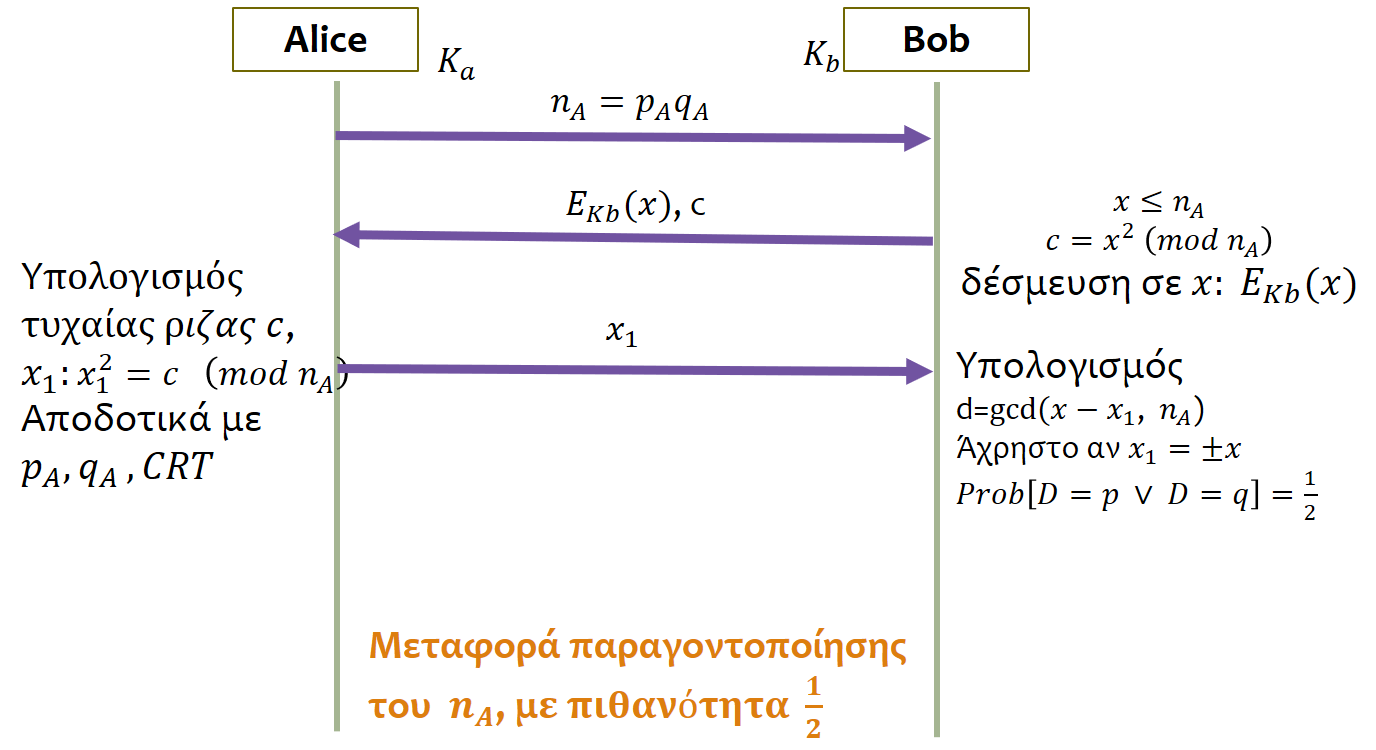
\includegraphics[scale=0.4]{rabinQR.png}
	\framebreak
	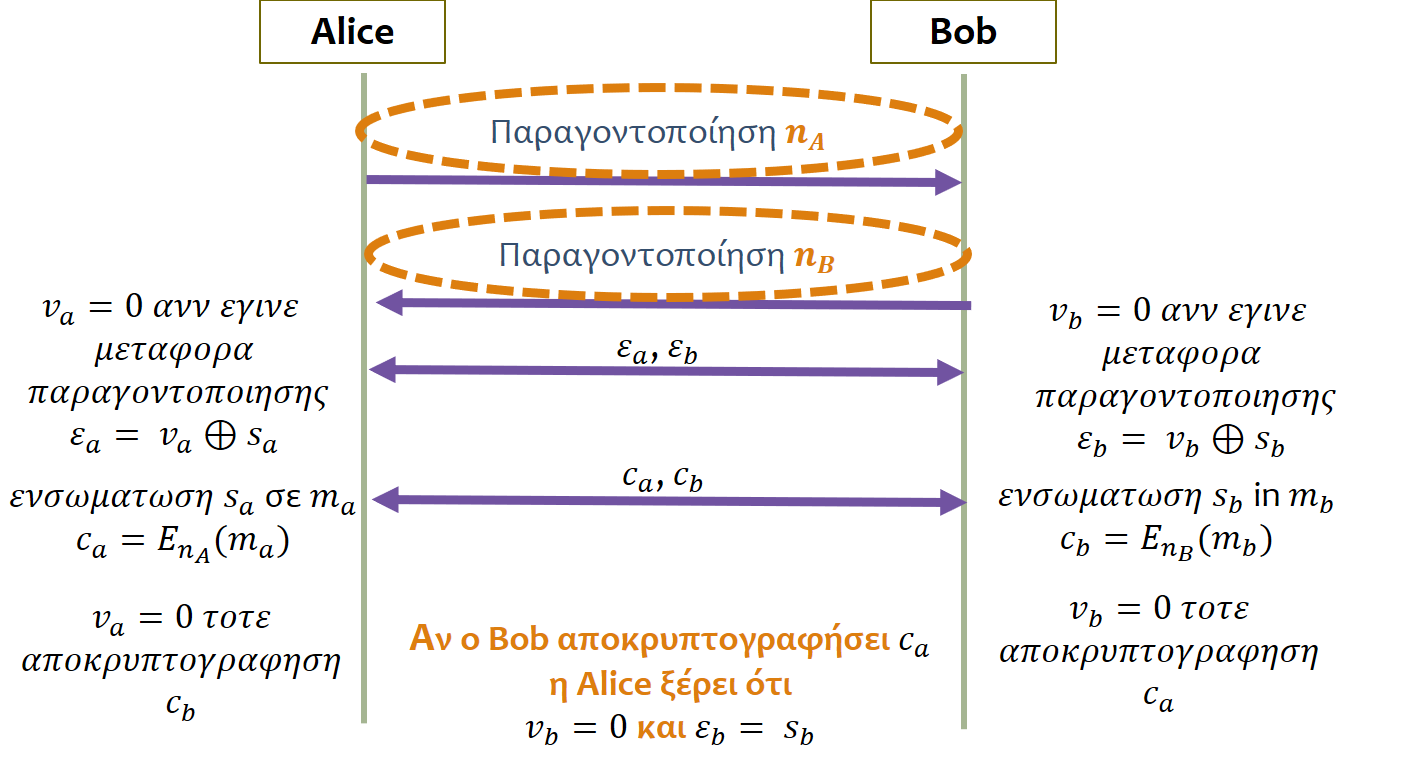
\includegraphics[scale=0.4]{rabinEOS.png}
\end{frame}

\begin{frame}{Γενίκευση: Μη συνειδητή μεταφορά (oblivious transfer)}
\begin{block}{Ορισμός $OT(S,R,M)$ (Even, Goldreich, Lempel)}
	Μη συνειδητή μεταφορά $OT(S,R,M)$ είναι ένα πρωτόκολλο με το οποίο ο αποστολέας $S$ μεταφέρει ένα μηνυμα $M$ στον παραλήπτη $R$ έτσι ώστε ο $R$ λαμβάνει το μήνυμα $Μ$ με πιθανότητα $1/2$ και:
	\begin{itemize}
		\item Αν ο $R$ δεν λάβει το μήνυμα, δεν μαθαίνει ούτε κάποια χρήσιμη πληροφορία
		\item Οποιαδήποτε προσπαθεια μη εκτέλεσης του πρωτοκόλλου γίνεται αντιληπτή
	\end{itemize}
\end{block}
Αφαιρετική αναπαράσταση καναλιού με θόρυβο
\end{frame}

\begin{frame}{Παραλλαγή: $1$-από-$2$ Μη-Συνειδητή Μεταφορά}
\begin{block}{$OT_1^2(S,R,$ $M_1,M_2)$}
	O $R$ επιλέγει μεταξύ δύο μηνυμάτων για μεταφορά με πιθανότητα ${1}/{2}$ και ο $S$ το μεταφέρει χωρίς ασφαλώς  να γνωρίζει ποιο μετέφερε. Μπορούμε να προσομοιώσουμε την τυχαία επιλογή χρησιμοποιώντας ένα bit.
\end{block}
\begin{figure}
	\centering
	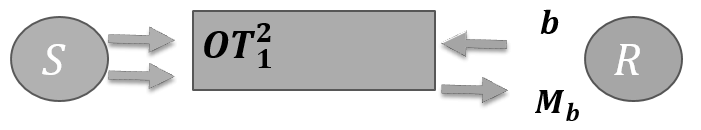
\includegraphics[width=0.8\textwidth]{ot12.png}
\end{figure}
\end{frame}

\begin{frame}{Άλλες παραλλαγές}
	\begin{block}{$OT_1^n(S,R,M_1,\cdots,M_n)$}
		O $R$ επιλέγει μεταξύ $n$ μηνυμάτων να λάβει το $i$. Φυσικά ο $S$ δεν το μαθαίνει, ενώ ο $R$ δεν μαθαίνει τα $M_j, j \neq i$
	\end{block}	

	$k$-από-$n$ Μη-Συνειδητή Μεταφορά
	\begin{itemize}
			\item O $R$ λαμβάνει ταυτόχρονα $k$ μηνύματα
			\item O $R$ λαμβάνει σειριακά $k$ μηνύματα που μπορούν να τροποποιηθούν με βάση τα προηγούμενα (adaptive)
	\end{itemize}
\end{frame} 

\begin{frame}{Πρακτική κατασκευή $OT_1^2$}
	\begin{itemize}
	\item Χρήση κρυπτοσυστήματος δημοσίου κλειδιού με $\mathcal{M} = \mathcal{C}$
	\item Τυχαία επιλογή  $x_0, x_1 \in \{0,1\}^*$ 
	\item Για να ληφθεί το $M_0$ ο $R$:
	\begin{itemize}
		\item Στέλνει στον $S$ το $(Enc(x_0),x_1)$
		\item Ο $S$ αποκρυπτογραφεί, παράγοντας το $(x_0, Dec(x_1))$.  
		\item Τελικά ο $S$ αποστέλλει το $(M_0 \xor x_0, M_1 \xor Dec(x_1))$
		\item Τελικά ο $R$ ανακτά το $M_0$ με XOR του πρώτου συστατικού: $M_0 \xor x_0 \xor x_0$
	\end{itemize}
	\end{itemize}
\end{frame}

\begin{frame}{Yao's Garbled Circuits}
	\begin{itemize}
		\item Χρήση $OT$ για κατασκευή κυκλώματος $C$ που υπολογίζει ασφαλώς ως προς παθητικό αντίπαλο μια συνάρτηση $f$
		\item Οι παίκτες παρέχουν στο $C$ τις εισόδους
		\item Mαθαίνουν το αποτέλεσμα χωρίς να αποκαλυφθεί οποιαδήποτε ενδιάμεση τιμή ή είσοδος
	\end{itemize}
	\begin{block}{Βασική ιδέα}
		Κατασκευή αλλοιωμένων πινάκων τιμών για τις λογικές πύλες του κυκλώματος με χρήση $OT$ 
	\end{block}
\end{frame}

\begin{frame}{Παράδειγμα: Πύλη OR}
	\begin{columns}
		\column{0.5\textwidth}
		\begin{itemize}
			\item Υπολογισμός $x = s$ $\mathtt{OR}$ $r$
			\item O $S$ παρέχει το $s$
			\item O $R$ παρέχει το $r$
		\end{itemize}
		\column{0.5\textwidth}
		\begin{figure}
			\centering
			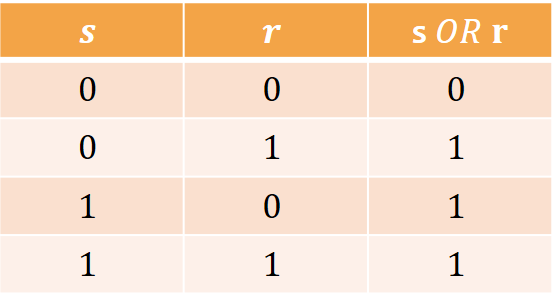
\includegraphics[width=\textwidth]{ot_or.png}
			\caption{Αρχικός πίνακας υπολογισμού OR}			 
		\end{figure}
	\end{columns}	
\end{frame}

\begin{frame}{Παράδειγμα: Garbled OR}
	\begin{columns}
		\column{0.55\textwidth}
		\begin{itemize}
			\item Επιλογή δύο τυχαίων μεταθέσεων $v_s, v_r : \{0,1\} \rightarrow \{0,1\} $ 
			\item Εφαρμογή στον πίνακα
			\item Επιλογή 4 ζευγών συναρτήσεων κρυπτογράφησης και αποκρυπτογράφησης 
			$(E_0^S, D_0^S), (E_1^S, D_1^S), (E_0^R, D_0^R), (E_1^R, D_1^R)$
			\item Εφαρμογή στο αποτέλεσμα της μετάθεσης
			\item Αποστολή στον $R$ μαζί με τη $v_r$
		\end{itemize}
		\column{0.45\textwidth}
		\begin{figure}
			\centering
			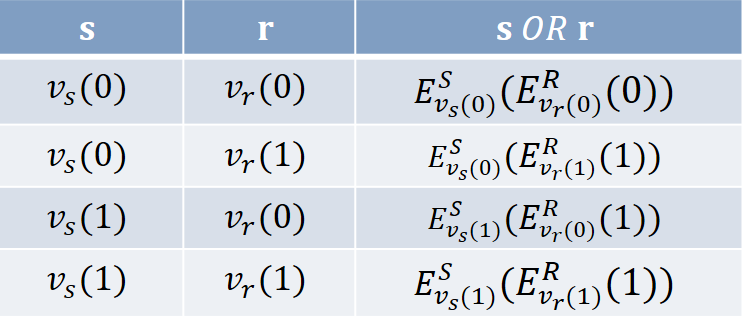
\includegraphics[width=1.2\textwidth]{ot_garbled_or.png}
			\caption{Αλλοιωμένος πίνακας υπολογισμού OR}
		\end{figure}
	\end{columns}	
\end{frame}

\begin{frame}{Υπολογισμός με Garbled OR}
	\begin{itemize}
		\item Ο $S$ υπολογίζει το $v_s(s)$ 
		\item Στέλνει στον $R$ το ζεύγος $(v_s(s),D_{v_s}^{S}(s))$
		\item O $R$ υπολογίζει το $v_r(r)$
		\item Για να αποκρυπτογραφήσει χρειάζεται την συνάρτηση $D_{(v_r(r))}^R$
		\item Πρέπει να την πάρει από τον $S$ \alert{χωρίς} να αποκαλυφθεί το $v_r(r)$
		\item Χρήση ${OT}_1^2(S,R,D_0^R,D_1^R)$
		\item Τελικά ο $R$ μπορεί να υπολογίσει το αποτέλεσμα $D^R_{v_r(r)}(D^S_{v_s(s)}(E^S_{v_s(s)}(E^R_{v_r(r)}(x))))$ και να το επιστρέψει στον $S$.
	\end{itemize}
\end{frame}

\begin{frame}{Γενίκευση}
	 
	\begin{itemize}
		\item Αλλοίωση όλων των πυλών
		\item Για κάθε πύλη
		\begin{itemize}
			\item  Mετάθεση γραμμών πίνακα αλήθειας $\rightarrow$ τυχαία μετάθεση αποτελέσματος
			\item  Θεώρουμε αποτέλεσμα και εισόδους ως τυχαία κλειδιά
			\item  Χρειάζονται 6 κλειδιά (4 είσοδοι - 2 αποτέλεσμα)
			\item  Υπολογισμός πύλης: γνώση κλειδιού αποτελέσματος
			\item  Τροφοδοσία επόμενης
		\end{itemize}		
		\item Οι τελικές έξοδοι αποκρυπτογραφούνται
	\end{itemize}
	 
\end{frame}

\begin{frame}[allowframebreaks]{Βιβλιογραφία}

\begin{tiny}
\begin{enumerate}
\item St. Zachos and Aris Pagourtzis. Στοιχεία Θεωρίας Αριθμών και Εφαρμογές στην Κρυπτογραφία. Πανεπιστημιακές Σημειώσεις
\item Jonathan Katz and Yehuda Lindell. Introduction to Modern Cryptography 2nd edition,  Chapman and Hall/CRC, 2015
\item Adi Shamir, \href{http://www5.in.tum.de/lehre/vorlesungen/konkr_math/WS_10_11/prog/shamir.pdf}{How to share a secret}.  Communications of the ACM 22.11 (1979): 612-613.
\item Helger Lipmaa, 79.159 Cryptography and Data Security, 24.03.2004 Lecture 9: Secret Sharing, Threshold Cryptography, MPC 
\item J. Kuhn \href{https://jeremykun.com/2014/06/23/the-mathematics-of-secret-sharing/}{The Mathematics of Secret Sharing}
\item M. Ben-Or, S. Goldwasser and A. Wigderson, “Completeness Theorems for Non-Cryptographic Fault-Tolerant Distributed Computation,” Proceedings of the 20th Annual ACM Symposium on Theory of Computing, Chicago, 1988, pp. 1-10.
\item Yao, A. C.  "Protocols for secure computations“ (FOCS 1982): 160–164
\item Rabin M. O. "How to exchange secrets by oblivious transfer." ,TR-81, Harvard University, 1981
\item S. Even, O. Goldreich, and A. Lempel. 1985. A randomized protocol for signing contracts. Commun. ACM 28, 6 (June 1985), 637-647
\item Claude Crépeau. 1987. Equivalence Between Two Flavours of Oblivious Transfers. In A Conference on the Theory and Applications of Cryptographic Techniques on Advances in Cryptology (CRYPTO '87, UK, 350-354.
\item Yehuda Lindell and Benny Pinkas. 2009. A Proof of Security of Yao’s Protocol for Two-Party Computation. J. Cryptol. 22, 2 (April 2009), 161-188
Ostrofski R., CS 282A/MATH 209A: Foundations of Cryptography, Lecture 10, Oblivious Transfer
\item Gabriel Bender, \href{http://www.math.uchicago.edu/~may/VIGRE/VIGRE2006/PAPERS/Bender.pdf}{Cryptography and Secure Two-Party Computation}, August 21, 2006
\item Ronald Cramer, Ivan Damgård, Jesper Buus Nielsen \href{https://pdfs.semanticscholar.org/6ae2/38ab990dd0c97fa972dc6087da7aaece4279.pdf}{Multiparty Computation, an Introduction} 
\end{enumerate}
\end{tiny}
\end{frame}

\end{document}
